\section{The Monte Carlo solution}\label{bsy:sec:mc}

\subsection{The vertical representation}

Write $f(\tau)=\log|\zeta(\theta+i\tau)|$ (or $\log|h|$ for another function) and $P=P_{1-\theta}(t_0-\cdot)$. The layer cake formula gives
\[
\E_P[f]=\int_0^\infty P(f>\lambda)\,d\lambda-\int_0^\infty P(f<-\lambda)\,d\lambda=:A^+-A^- .
\]
In this vertical form Theorem~\ref{bsy:thm:bsy} says that $\mathrm{QRH}(\theta)$ holds exactly when the upper and lower tail areas of $\log|\zeta|$ under harmonic measure differ by $\log|h_\theta(1+it_0)|$, for one (equivalently every) $t_0$. The lower tail $P(f<-\lambda)$ is the harmonic measure of the neighbourhoods $\{|\zeta|<e^{-\lambda}\}$ of the zeros on the line, which decays like $e^{-\lambda}$ when $\theta=\frac12$ and the zeros are simple (heuristic on the whole line).

\begin{lemma}[finite moments]\label{bsy:lem:var}
For $\frac12\le\theta<1$, every $t_0$ and every $p<\infty$, $\E_P[|f|^p]<\infty$. Hence plain Monte Carlo with exact Cauchy draws is unbiased, needs no truncation of the heavy tail, and has root mean square error $(\mathrm{Var}_Pf/n)^{1/2}$.
\end{lemma}

\begin{proof}
The density of $P$ is $\ll_{t_0}(1+t^2)^{-1}$, $|\zeta(\theta-it)|=|\zeta(\theta+it)|$, and $f$ has only logarithmic singularities on bounded intervals, so $\int_{-2}^2|f|^p\,dP<\infty$, and it suffices to show $\int_T^{T+1}|f(t)|^p\,dt\ll_p\log^pT$ for $T\ge2$, since $\sum_TT^{-2}\log^pT<\infty$. By the convexity bound, $\log^+|\zeta(\theta+it)|\ll\log T$ on $[T,T+1]$. By the local formula $\log|\zeta(s)|=\sum_{|\gamma-t|\le1}\log|s-\rho|+O(\log t)$, uniform in $-1\le\sigma\le2$ \cite[Chapter IX]{Titchmarsh}, and $|\theta+it-\rho|\ge|t-\gamma|$,
\[
\log^-|\zeta(\theta+it)|\le\sum_{|\gamma-t|\le1}\log^-|t-\gamma|+O(\log T).
\]
The number $n_T$ of zeros with $|\gamma-T|\le2$ is $O(\log T)$. By H\"older's inequality for the sum over $n_T$ terms,
\[
\int_T^{T+1}\Bigl(\sum_{|\gamma-t|\le1}\log^-|t-\gamma|\Bigr)^p\,dt\le n_T^{\,p-1}\sum_{|\gamma-T|\le2}\int_{\R}\bigl(\log^-|x|\bigr)^p\,dx\ll_p\log^pT,
\]
since $\int_{\R}(\log^-|x|)^p\,dx=2\,\Gamma(p+1)$.
\end{proof}

\subsection{Three estimators}

\paragraph{Quadrature} Adaptive Gauss quadrature on $|\tau-t_0|\le W$, with the zeros on the line used as breakpoints so that the logarithmic singularities are endpoint singularities. The neglected Cauchy mass is $\frac2\pi\arctan\frac{1-\theta}W\approx\frac{2(1-\theta)}{\pi W}$; the neglected part of the integral needs its own bound (Cauchy and Schwarz with Lemma~\ref{bsy:lem:var}).

\paragraph{Plain Monte Carlo} Draw $\tau_i=t_0+(1-\theta)\tan\bigl(\pi(u_i-\frac12)\bigr)$ with $u_i$ uniform, and average $f(\tau_i)$. Lemma~\ref{bsy:lem:var} makes this unbiased with a finite standard error.

\paragraph{Vertical likelihood Monte Carlo} Following Polson and Scott \cite{VLMC14}, sample instead from a law that reweights the levels of $f$,
\[
P_w(d\tau)\ \propto\ P(d\tau)\,w\bigl(f(\tau)\bigr),
\]
and recover $\E_P[f]$ and the vertical curves $P(f>\lambda)$, $P(f<-\lambda)$ by self normalised weights $1/w$. We use $w(f)=|f-c|+\epsilon$, with $c$ a pilot estimate, a regularised form of the weight $|f-\E_Pf|$, which is optimal for independent draws (Remark~\ref{bsy:rem:weight}). We sample $P_w$ by a Metropolis chain mixing Cauchy independence proposals with local moves. The weighting visits the deep levels $\{f<-\lambda\}$ near the zeros and the upper tail more often than plain sampling (computed, Table~\ref{bsy:tab:defects} and below).

\begin{remark}[the optimal weight]\label{bsy:rem:weight}
Let $\mu=\E_Pf$, $w>0$, $Z=\E_Pw$ and $q=Pw/Z$. For independent draws $\tau_i\sim q$ the self normalised estimator $\hat\mu=\sum_if(\tau_i)/w(\tau_i)\big/\sum_i1/w(\tau_i)$ satisfies $n\,\mathrm{Var}(\hat\mu)\to Z\,\E_P[(f-\mu)^2/w]$, since $\hat\mu-\mu=Z\,n^{-1}\sum_i(f-\mu)(\tau_i)/w(\tau_i)+o_P(n^{-1/2})$ and $\E_q[(f-\mu)^2/w^2]=Z^{-1}\E_P[(f-\mu)^2/w]$. By the Cauchy and Schwarz inequality the limit is at least $(\E_P|f-\mu|)^2$, with equality exactly for $w\propto|f-\mu|$, and $(\E_P|f-\mu|)^2\le\mathrm{Var}_Pf$, with equality only if $|f-\mu|$ is constant. So for independent draws the weight $|f-\mu|$, the standard optimal proposal of self normalised importance sampling, strictly beats plain Monte Carlo for these integrands, and $|f-c|+\epsilon$ approximates it. For the integrands of Table~\ref{bsy:tab:defects} the factor $\mathrm{Var}_Pf/(\E_P|f-\mu|)^2$ ranges over the nine rows from $1.35$ (DH, $\theta=\frac34$, $t_0=85.7$) to $2.46$ ($\zeta$, $\theta=\frac78$, $t_0=85.7$; the nine values are $1.35$, $1.41$, $1.43$, $1.48$, $1.55$, $1.86$, $2.02$, $2.13$ and $2.46$), with an error of up to $0.03$ (computed by quadrature), so for independent draws no weight gains more than that. For a Markov chain the limit is $Z^2\bigl[\mathrm{Var}_qY_0+2\sum_{j\ge1}\mathrm{Cov}_q(Y_0,Y_j)\bigr]$ with $Y=(f-\mu)/w$, when a central limit theorem holds; negative autocorrelation can bring it below the value for independent draws.
\end{remark}

\subsection{Results}

Table~\ref{bsy:tab:defects} reports the local defect $D_\theta(t_0)$ for $\zeta$ and for the Davenport and Heilbronn function (with $h=f$, which is entire), whose zero $0.808517182457+85.699348485378\,i$ lies off the line (certified in Section~\ref{cf:sec:test}; see also \cite{Spira94,BSO07}). The prediction for $\zeta$ is zero, under RH for $\theta=\frac12$ and under $\mathrm{QRH}(\theta)$ for the other levels. For Davenport and Heilbronn it is the sum of the Green potentials of its zeros with $\beta>\theta$, at least that of this zero (the other zeros below height $200$ add about $2\times10^{-4}$ at $\theta=\frac12$ and less than $10^{-5}$ at $\theta=\frac34$): $\log(0.8085/0.1915)\approx1.440$ at $\theta=\frac12$ and $\log(0.3085/0.1915)\approx0.477$ at $\theta=\frac34$.

\begin{table}[h]
\centering\scriptsize\setlength{\tabcolsep}{2pt}
\begin{tabular}{lccccc}
\toprule
$(\theta,t_0)$ & prediction & quad.\ $W=60$ & quad.\ $W=200$ & plain MC & vertical MC\\
\midrule
$\zeta$ $(\frac12,0)$ & $0$ & $-4.1\times10^{-5}$ & $5.0\times10^{-6}$ & $-0.0040\pm0.0026$ & $-0.0021\pm0.0055$\\
$\zeta$ $(\frac78,0)$ & $0$ & $-7.9\times10^{-6}$ & $8.7\times10^{-7}$ & $-0.0032\pm0.0049$ & $-0.0173\pm0.0132$\\
$\zeta$ $(\frac12,85.7)$ & $0$ & $1.79\times10^{-4}$ & $-1.5\times10^{-6}$ & $-0.0146\pm0.0061$ & $-0.0064\pm0.0141$\\
$\zeta$ $(\frac34,85.7)$ & $0$ & $5.8\times10^{-5}$ & $-7.9\times10^{-7}$ & $-0.0022\pm0.0026$ & $-0.0074\pm0.0055$\\
$\zeta$ $(\frac78,85.7)$ & $0$ & $2.2\times10^{-5}$ & $-3.8\times10^{-7}$ & $-0.0011\pm0.0016$ & $0.0037\pm0.0032$\\
DH $(\frac12,85.7)$ & $1.4407$ & $1.4405$ & $1.4406$ & $1.4374\pm0.0133$ & $1.4727\pm0.0229$\\
DH $(\frac34,85.7)$ & $0.4770$ & $0.47697$ & $0.47698$ & $0.4759\pm0.0159$ & $0.4740\pm0.0312$\\
DH $(\frac34,100)$ & $1.49\times10^{-4}$ & $1.16\times10^{-4}$ & $1.47\times10^{-4}$ & $0.0099\pm0.0054$ & $0.0139\pm0.0130$\\
DH $(\frac78,85.7)$ & $0$ & $-3.8\times10^{-6}$ & $-3.6\times10^{-7}$ & $-0.0160\pm0.0141$ & $-0.0311\pm0.0260$\\
\bottomrule
\end{tabular}
\caption{Local defects $D_\theta(t_0)$ (computed, floating point). Davenport and Heilbronn is abbreviated DH. The quadrature columns are the integral over $|\tau-t_0|\le W$ minus $\log|h_\theta(1+it_0)|$, with the zeros as breakpoints: they are realised truncation errors of the window, not accuracies, and change with $W$. Outside the window the Cauchy mass is $0.0053$ at $\theta=\frac12$, $0.0027$ at $\theta=\frac34$ and $0.0013$ at $\theta=\frac78$ for $W=60$. Monte Carlo (computed) uses $n=20{,}000$ evaluations for $\zeta$ and $4{,}000$ for DH. Plain Monte Carlo uses exact Cauchy draws, with standard error $\mathrm{sd}/\sqrt n$. The vertical sampler takes a pilot mean $c$ from $n/20$ draws, $\epsilon=0.05$ times the standard deviation of the pilot, an even mixture of Cauchy independence proposals and Gaussian steps of scale $(1-\theta)/2$, and a burn in of $n/20$ steps, with batch means standard errors ($50$ batches). The Davenport and Heilbronn prediction is the sum of the Green potentials of the zeros found below height $700$; for $\theta=\frac78$ none has $\beta>\frac78$, but $f$ has zeros with $\beta>1$ \cite{DH36}, so the exact defect is positive.}\label{bsy:tab:defects}
\end{table}

The quadrature values agree with the predictions to the size of the neglected tail, which is larger than the printed values suggest. For $\zeta$ at $(\frac12,0)$ the Cauchy and Schwarz bound for the neglected part, over blocks of unit length, is $5.3\times10^{-3}$ (computed up to height $1000$) plus $1.1\times10^{-3}$ (extrapolated, heuristic) at $W=60$, and $1.4\times10^{-3}$ plus $1.1\times10^{-3}$ at $W=200$; at $(\frac78,0)$ it is $6.3\times10^{-4}$ plus $1.7\times10^{-4}$ and $1.6\times10^{-4}$ plus $1.7\times10^{-4}$; for Davenport and Heilbronn at $(\frac34,85.7)$ it is $1.0\times10^{-3}$ plus $6.2\times10^{-4}$ and $2.0\times10^{-4}$ plus $6.2\times10^{-4}$. The two Monte Carlo columns agree with the quadrature values within $2.4$ standard errors (plain Monte Carlo for $\zeta$ at $(\frac12,85.7)$ is $2.4$ off, the other seventeen entries are within $2$), and at height $100$ neither sampler resolves the defect $1.49\times10^{-4}$, which is far below their standard errors $0.005$ and $0.013$. The local character of the criterion is visible in the last rows: centred at the zero the defect of Davenport and Heilbronn at $\theta=\frac34$ is the order one number $0.477$, and seen from height $100$ the same zero gives $1.4\times10^{-4}$.

At $\theta=\frac78$ and $t_0=0$ the criterion of Theorem~\ref{bsy:thm:bsy} reads
\[
\frac1\pi\int_{-\infty}^{\infty}\log|\zeta(\tfrac78+i\tau)|\,\frac{1/8}{1/64+\tau^2}\,d\tau=\log4+D_{7/8}(0),
\]
with $D_{7/8}(0)=0$ under $\mathrm{QRH}(\frac78)$; the quadrature gives $\log4$ to within the window error of the table. With no hypothesis, each zero with $\beta>\theta$ adds at most $2(1-\theta)(\beta-\theta)/\gamma^2$ to $D_\theta(0)$, and by Remark~\ref{bsy:rem:local} all possible zeros above the verified height add less than $10^{-12}$ at every level (computed). The global criterion is therefore numerically blind above the verified range and useful only locally.

All three estimators agree with the predictions. Quadrature gives the smallest realised errors, with the caveat above. Plain Monte Carlo has the smaller standard error of the two samplers; the vertical sampler pays for its Markov dependence and its importance weights, and buys more visits to the deep levels: at $\theta=\frac12$ it visits $\{f<-2\}$ more often (computed: $315$ visits against $25$ for $\zeta$ at $(\frac12,0)$, $2952$ against $679$ at $(\frac12,85.7)$, $76$ against $43$ for Davenport and Heilbronn), without reaching a deeper minimum of $f$.

Figure~\ref{bsy:fig:vertical} shows the vertical picture. For $\zeta$ the running balance $A^+(\Lambda)-A^-(\Lambda)-\log|h(1+it_0)|$ settles at zero once the level cutoff passes about $4$. For Davenport and Heilbronn it settles near the Green potential $1.44$ of the zero off the line.

\begin{figure}[h]
\centering
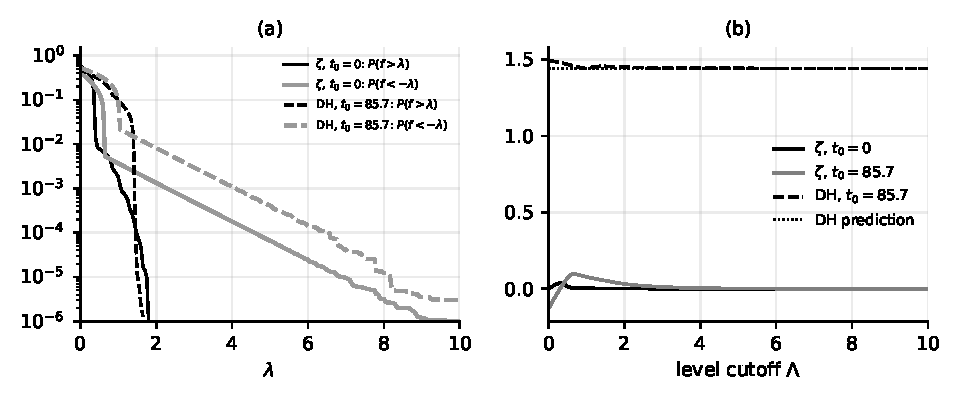
\includegraphics[width=\textwidth]{fig/bsy_vertical.pdf}
\caption{Vertical curves at $\theta=\frac12$ (computed, floating point). Left: $P(f>\lambda)$ (black) and $P(f<-\lambda)$ (grey) under the Cauchy law centred at $t_0$, for $\zeta$ at $t_0=0$ (solid) and Davenport and Heilbronn at $t_0=85.7$ (dashed), $\lambda\le10$, logarithmic vertical axis. Right: the running balance $\E[\mathrm{clip}(f,-L,L)]-\log|h(1+it_0)|$, which converges to the defect $D_{1/2}(t_0)$, for $\zeta$ at $t_0=0$ and $85.7$ and for Davenport and Heilbronn at $t_0=85.7$, with the prediction $1.4407$ dotted; window $|\tau-t_0|\le200$, neglected Cauchy mass $0.0016$.}\label{bsy:fig:vertical}
\end{figure}

\subsection{Weighted Monte Carlo of Yakowitz, Krimmel and Szidarovszky}

The map $\tau(u)=t_0+a\tan\bigl(\pi(u-\frac12)\bigr)$, with $a=1-\theta$, writes every Cauchy average as an integral over the unit interval, $\E_P[f]=\int_0^1g(u)\,du$ with $g=f\circ\tau$. Yakowitz, Krimmel and Szidarovszky \cite{YKS78} proposed sorting uniform nodes $u_{(1)}<\dots<u_{(N)}$ and applying the trapezoid rule:
\[
T_N=\sum_{i=0}^{N}\bigl(u_{(i+1)}-u_{(i)}\bigr)\,\frac{g(u_{(i)})+g(u_{(i+1)})}{2},\qquad u_{(0)}=0,\ u_{(N+1)}=1 .
\]
We set $g(0)=g(1)=0$, a convention: $g$ has no limit at the ends, and $0$ is the mean of $\log|\zeta|$ on the line $\Re s=\theta$ for $\theta>\frac12$, and for $\theta=\frac12$ under RH. Their theorem: if $g\in C^2[0,1]$ then $\E(T_N-\E_P f)^2=O(N^{-4})$, against $O(N^{-1})$ for the sample mean. Lemma~\ref{bsy:lem:trap} below gives the leading bias. The same weights define a rule for any node set, so the states of the vertical likelihood chain can serve as nodes, the spacings replacing the weights $1/w$, although the theorem does not transfer to dependent nodes.

The spacings remove the variance that the sample mean spends on the smooth part of $g$, and the Euler product supplies a second, exact reduction.

\begin{lemma}[exact Cauchy means]\label{bsy:lem:cv}
For any Dirichlet polynomial $D(s)=\sum_{n\le M}b_nn^{-s}$ and $a=1-\theta$,
\[
\begin{gathered}
\E_P\bigl[\Re D(\theta+i\tau)\bigr]=\Re D(1+it_0),\\
\E_P\Bigl[\log\Bigl|\frac{\theta+1+i\tau}{\theta-1+i\tau}\Bigr|\Bigr]=\log\Bigl|\frac{2+it_0}{2-2\theta+it_0}\Bigr| .
\end{gathered}
\]
\end{lemma}

\begin{proof}
The characteristic function of the Cauchy law gives $\E_P[n^{-i\tau}]=n^{-it_0}e^{-a\log n}$, so each term $n^{-\theta-i\tau}$ averages to $n^{-1-it_0}$. For the second, $|\theta-1+i\tau|=|\theta-(2\theta-1)+i\tau|$ on the line, and $\log|s+1|-\log|s-2\theta+1|$ is harmonic on $\{\Re s>\theta\}$; its Poisson integral at $1+it_0$ is its value there.
\end{proof}

With $D_M$ the Selberg smoothed truncation of $\log\zeta$, $b_n=\frac{\Lambda(n)}{\log n}\bigl(1-\frac{\log n}{\log M}\bigr)$, we apply the trapezoid rule to $g-\Re D_M\circ\tau-\ell\circ\tau$, where $\ell$ is the pole term of Lemma~\ref{bsy:lem:cv}, and add back the exact means. Table~\ref{bsy:tab:yks} and Figure~\ref{bsy:fig:yks} report root mean square errors over $400$ replications, at $t_0=0$, against the values $0$ and $\log4$ that the criterion gives under RH and $\mathrm{QRH}(\frac78)$; with no hypothesis they hold to within $7.4\times10^{-13}$ and $4.7\times10^{-14}$ (Remark~\ref{bsy:rem:local}).

\begin{table}[h]
\centering\small
\begin{tabular}{cccccc}
\toprule
$\theta$ & $N$ & plain & YKS & YKS with control & gain\\
\midrule
$\tfrac12$ & 500 & $1.7\times10^{-2}$ & $9.6\times10^{-3}$ & $5.3\times10^{-3}$ & 3.2\\
$\tfrac12$ & 2000 & $8.4\times10^{-3}$ & $4.0\times10^{-3}$ & $2.6\times10^{-3}$ & 3.3\\
$\tfrac12$ & 8000 & $4.2\times10^{-3}$ & $1.6\times10^{-3}$ & $1.1\times10^{-3}$ & 3.7\\
$\tfrac12$ & 16000 & $3.1\times10^{-3}$ & $9.7\times10^{-4}$ & $7.2\times10^{-4}$ & 4.3\\
$\tfrac78$ & 500 & $3.0\times10^{-2}$ & $2.3\times10^{-3}$ & $4.0\times10^{-4}$ & 74\\
$\tfrac78$ & 2000 & $1.5\times10^{-2}$ & $1.3\times10^{-3}$ & $2.3\times10^{-4}$ & 65\\
$\tfrac78$ & 8000 & $7.7\times10^{-3}$ & $4.8\times10^{-4}$ & $1.0\times10^{-4}$ & 75\\
$\tfrac78$ & 16000 & $5.1\times10^{-3}$ & $2.9\times10^{-4}$ & $6.9\times10^{-5}$ & 75\\
\bottomrule
\end{tabular}
\caption{Root mean square error of the Cauchy average of $\log|\zeta(\theta+i\tau)|$, $t_0=0$, over $400$ replications (computed, floating point; the sampling error of each entry is about $3.5\%$ and larger for the heavy tailed plain estimator). The control uses $M=100$ at $\theta=\frac12$ and $M=1000$ at $\theta=\frac78$. Gain is the ratio of plain to YKS with control. Fitted slopes over $500\le N\le16{,}000$ at $\theta=\frac12$ and $\frac78$: plain $-0.49$ and $-0.50$, YKS $-0.66$ and $-0.60$, YKS with control $-0.58$ and $-0.52$.}\label{bsy:tab:yks}
\end{table}

\begin{figure}[h]
\centering
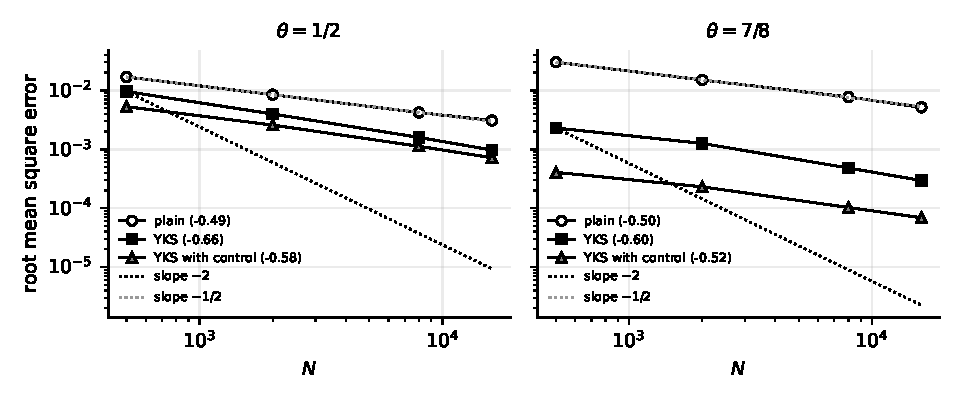
\includegraphics[width=\textwidth]{fig/bsy_yks_rates.pdf}
\caption{Root mean square error against $N$ (from the $400$ replications of Table~\ref{bsy:tab:yks}), drawn for $\theta=\frac12$ and $\frac78$ for plain sampling, YKS and YKS with control, with the fitted slopes in the legend. The dotted lines have slope $-2$ (anchored at the first YKS point), the rate of the theorem of Yakowitz, Krimmel and Szidarovszky for integrands in $C^2[0,1]$, and slope $-\frac12$ (anchored at the first plain point).}\label{bsy:fig:yks}
\end{figure}

At $\theta=\frac78$ the trapezoid weights alone reduce the error by a factor between $12$ and $18$, and with the control by a factor between $65$ and $75$, equivalent to between $4{,}000$ and $6{,}000$ times as many plain samples. At $\theta=\frac12$ the factor is between $3$ and $4.3$. With coefficient one the control alone makes the sample mean worse: over $400$ replications its root mean square error is $3.3$ times that of plain sampling at $\theta=\frac12$ and $1.04$ times at $\theta=\frac78$ (computed); it helps only once the trapezoid weights have removed the variance of the smooth part.

The rate, however, is not $N^{-2}$: the fitted slopes over $500\le N\le16{,}000$ lie between $-0.49$ and $-0.66$ for every method. The hypothesis $g\in C^2[0,1]$ fails, and indeed $g\notin C^1[0,1]$:

\begin{proposition}[why the $N^{-4}$ bound does not apply]\label{bsy:prop:rate}
Let $\frac12\le\theta<1$, $f(\tau)=\log|\zeta(\theta+i\tau)|$ and $g=f\circ\tau$. If $\theta=\frac12$, $g$ is unbounded near $\tau^{-1}(\gamma)$ for every ordinate $\gamma$ of a zero on the line. If $\frac12<\theta<1$, $g'$ is unbounded near $u=0$ and near $u=1$. In both cases $g\notin C^1[0,1]$.
\end{proposition}

\begin{proof}
For $\theta=\frac12$, $f(\tau)\to-\infty$ as $\tau\to\gamma$. Let $\frac12<\theta<1$ and suppose $|g'|\le C$ on $(1-\eta,1)$. Then $g(u)$ has a limit as $u\to1$, so $|\zeta(\theta+i\tau)|\to e^L$ for some $L$ as $\tau\to\infty$. The mean value theorems for $\sigma>\frac12$ \cite[Chapter VII]{Titchmarsh} give $T^{-1}\int_1^T|\zeta(\theta+it)|^2dt\to\zeta(2\theta)$ and $T^{-1}\int_1^T|\zeta(\theta+it)|^4dt\to\zeta(2\theta)^4/\zeta(4\theta)$, so $e^{2L}=\zeta(2\theta)$ and $e^{4L}=\zeta(2\theta)^4/\zeta(4\theta)$, whence $\zeta(2\theta)^2=\zeta(4\theta)$. This is false, since $\zeta(4\theta)=\sum_{n=m^2}n^{-2\theta}<\sum_nd(n)\,n^{-2\theta}=\zeta(2\theta)^2$. The end $u=0$ is the same, because $|\zeta(\theta-i\tau)|=|\zeta(\theta+i\tau)|$.
\end{proof}

\begin{remark}[a heuristic rate]
For a single component $f(\tau)=\cos(k\tau)$ the following count suggests a mean square error of order $\sqrt{ak}\,N^{-3/2}$ for the sorted trapezoid rule, that is a root mean square error of order $N^{-3/4}$ (heuristic). Near $u=1$, $\tau-t_0\approx a/(\pi(1-u))$, and $\tau'(u)=\pi\bigl(a^2+(\tau-t_0)^2\bigr)/a$. A cell of width $h\approx1/N$ in $u$ has width $\Delta\approx h\pi(\tau-t_0)^2/a$ in $\tau$ for large $\tau$. Cells with $k\Delta\lesssim1$ contribute variance of order $h^2(k\Delta)^4$; cells beyond $T_N\asymp(aN/k)^{1/2}$, where $k\Delta\gtrsim1$, behave like independent samples and contribute of order $h^2$ each. There are about $Na/(\pi\tau^2)$ cells per unit of $\tau$. The two sums are each of order $\sqrt{ak}\,N^{-3/2}$.
\end{remark}

A test with $f(\tau)=\cos(\tau\log2)$ gives the slope $-0.74$ for the trapezoid rule at both levels over $500\le N\le128{,}000$ (and $-0.50$ for plain sampling), close to the predicted $-\frac34$. The Selberg smoothed polynomials $\Re D_{1000}$ give $-0.67$ at $\theta=\frac78$ and $-0.71$ at $\theta=\frac12$. The true integrands give $-0.60$ and $-0.66$ for the trapezoid rule alone, and only the plain slope is near $-\frac12$. The likely cause (heuristic) is the features that the polynomial lacks: the logarithmic singularity at each zero on the line, and the dips of width $\theta-\frac12$ at the heights of the zeros, whose number grows like $\log\tau$. Each of these adds error at the scale of one cell.

Nor does the $N^{-4}$ rate transfer to the vertical scale. First, the vertical representation needs the masses $X(\lambda)=P(f<-\lambda)$ at the nodes. In nested sampling and in the vertical likelihood chain these are estimated, with a Monte Carlo error (of order $N^{-1/2}$ for independent draws) that a better quadrature rule alone does not remove (heuristic). Second, even computed exactly, the quantile function of $f$ under $P$ has a logarithmic singularity at $0$ when $\theta=\frac12$, because $P(f<-\lambda)\asymp e^{-\lambda}$ (heuristic, as above), and a flat point at every nondegenerate critical value of $f$, where the law of $f$ has an inverse square root singularity, one for each gap between consecutive zeros. Whether the vertical chain's visited states, which concentrate nodes at the deep levels and leave wider gaps elsewhere, work as nodes of the trapezoid rule is not tested here; its error is governed by the widest gaps where $g$ oscillates (heuristic).

In one dimension, quadrature with the zeros as breakpoints remains the method of choice. The Yakowitz weights with the Dirichlet control are for averages that quadrature cannot reach cheaply, such as double integrals over level and height, where the trapezoid rule becomes the Voronoi and Delaunay rules (Section~\ref{bsy:sec:2d}).

\subsection{An exact identity on a half disc}\label{bsy:sec:halfdisk}

Whether another parametrisation of the whole line gives an integrand smooth enough for the rates of Yakowitz, Krimmel and Szidarovszky is not settled here: for a positive integrand the distribution function of $fP$ makes the transformed integrand constant, but it needs the integral itself. A change of domain does work. Cut the line at the heights $t_0\pm R$ and close the contour by a semicircle in the half plane, where $\log|h|$ is harmonic away from the zeros; the Cauchy weight becomes the harmonic measure of a half disc, and the identity stays exact.

\begin{theorem}[Balazard, Saias and Yor on a half disc]\label{bsy:thm:halfdisk}
Let $c=\theta+it_0$, $R>0$, $H=\{|s-c|<R,\ \Re s>\theta\}$, $z\in H$, and let $\omega_z$ be the harmonic measure of $\partial H$ seen from $z$. Let $h\not\equiv0$ be analytic on a neighbourhood of $\overline H$, with no zero on the closed arc $\{|s-c|=R,\ \Re s\ge\theta\}$, with zeros $\rho_1,\dots,\rho_n$ of multiplicities $m_1,\dots,m_n$ on the open diameter, and with $h(z)\ne0$. Then
\[
\begin{aligned}
\int_{\partial H}\Bigl(\log|h|-\sum_jm_j\log|s-\rho_j|\Bigr)\,d\omega_z
&=\log|h(z)|-\sum_jm_j\log|z-\rho_j|\\&\quad+\sum_{\rho\in H}G_H(z,\rho),
\end{aligned}
\]
the last sum over the zeros of $h$ in $H$ with multiplicity, and the integrand on the left is real analytic on each of the two closed pieces of $\partial H$. In the coordinate $w=(s-c)/R$, with $w_z=(z-c)/R$, $w^*=-\overline{w_z}$ the reflection of $w_z$ in the diameter and $G_D(a,w)=\log|(1-\bar aw)/(w-a)|$,
\[
G_H(z,\cdot)=G_D(w_z,\cdot)-G_D(w^*,\cdot),\]\[
\frac{d\omega_z}{d\phi}=\frac{1-|w_z|^2}{2\pi|e^{i\phi}-w_z|^2}-\frac{1-|w^*|^2}{2\pi|e^{i\phi}-w^*|^2}
\]
on the arc $w=e^{i\phi}$, $|\phi|\le\frac\pi2$, and on the diameter $w=iy$, $|y|\le1$, the density with respect to $dy$ is $\frac1{2\pi}\partial_x\bigl[G_D(w_z,x+iy)-G_D(w^*,x+iy)\bigr]$ at $x=0$. Both densities are real analytic up to the corners $w=\pm i$, where they vanish to first order. In particular $h$ has no zero in $H$ if and only if the identity holds without the Green sum.
\end{theorem}

\begin{proof}
Put $q(s)=h(s)\prod_j(s-\rho_j)^{-m_j}$. Then $q$ is analytic on a neighbourhood of $\overline H$ with no zero on $\partial H$, so $\log|q|=\log|h|-\sum_jm_j\log|s-\rho_j|$ is real analytic on a neighbourhood of $\partial H$. Green's identity on $H$ with small discs about the zeros of $q$ removed (on the circle of radius $r$ about a zero of multiplicity $m$ the normal derivative of $\log|q|$ integrates to $2\pi m+O(r)$) gives the Riesz decomposition $\log|q(z)|=\int_{\partial H}\log|q|\,d\omega_z-\sum_{\rho\in H}G_H(z,\rho)$, which is the identity. The function $G_D(w_z,\cdot)-G_D(w^*,\cdot)$ vanishes on the unit circle and, because $w^*$ is the reflection of $w_z$ in the imaginary axis, on the diameter, and its only singularity in the half disc is the logarithmic pole at $w_z$; so it is the Green function of $H$. The harmonic measure density is its inner normal derivative divided by $2\pi$, which gives the two formulas. They are rational in the boundary point, and at the right angled corners $w=\pm i$ each has a simple zero, as the reflection principle predicts. Since $G_H>0$ on $H$, the Green sum vanishes exactly when $H$ contains no zero.
\end{proof}

\begin{remark}[the half plane as a limit]\label{bsy:rem:halfplane}
Let $h=h_\theta$ and $z=1+it_0$. Each $\log|s-\rho_j|$ is the Poisson integral of its boundary values (it is the real part of $\log(s-\rho_j)$, which lies in $H^p$ of the half plane for every $p<\infty$), so the identity also holds with the subtracted terms removed on both sides. As $R\to\infty$ the density on the diameter increases to the Cauchy density $P_{1-\theta}(t_0-\cdot)$, since harmonic measure on the common boundary increases with the domain, and the Green sum increases to the sum of Theorem~\ref{bsy:thm:bsy}. On the arc the density is at most $CR^{-1}\cos\phi$, so the part of the arc in $\theta\le\Re s\le2$ has harmonic measure $O(R^{-3})$; along radii $R_k\to\infty$ with $|t_0\pm R_k-\gamma|\ge c/\log R_k$ for every zero, $|\log|h_\theta||=O(\log^2R_k)$ there, while $|\log|h_\theta(s)||=O(2^{-\Re s}+R_k^{-1})$ on the rest of the arc. So the arc term tends to $0$, and with Lemma~\ref{bsy:lem:var} and dominated convergence on the diameter Theorem~\ref{bsy:thm:halfdisk} becomes Theorem~\ref{bsy:thm:bsy} at $1+it_0$. That the arc carries vanishing harmonic measure would not suffice by itself: for $h(s)=e^{s-\theta}$ the arc contributes $1-\theta$ for every $R$.
\end{remark}

Wunderlich \cite{Wun26} gives other finite radius forms of the criterion, by Jensen's formula on discs with the trivial zeros removed explicitly, and a relative entropy form: if $X$ has the density $6/(\pi(1+t^2)(4+t^2))$, which is twice the Cauchy$(0,1)$ density minus the Cauchy$(0,2)$ density, $\Xi(t)=\xi(\frac12+it)$ is Riemann's Xi function, $\E\log|\Xi(X)|$ is finite, $W=|\Xi(X)/\Xi(0)|^2$, and $\nu$ is the law with density $W/\E W$ with respect to the law $\lambda$ of $X$, then $D_{\mathrm{KL}}(\lambda\|\nu)=\log\E W-\E\log W$, with no hypothesis; in his formulation RH is the saturation of a separate bound.

\begin{lemma}[the sorted trapezoid rule]\label{bsy:lem:trap}
Let $g\in C^4[a,b]$ and let $T_N$ be the sorted trapezoid rule at $N$ independent uniform nodes on $[a,b]$ with the end points added, as in Section~\ref{bsy:sec:mc} (there $g$ vanishes at the end points, here its end values are used). Then
\[
\E T_N-\int_a^bg=\frac{(b-a)^2\bigl(g'(b)-g'(a)\bigr)}{2(N+1)(N+2)}+O(N^{-3}),\qquad\mathrm{Var}\,T_N=O(N^{-5}).
\]
So the mean square error is $O(N^{-4})$, and $O(N^{-5})$ when $g'(a)=g'(b)$.
\end{lemma}

\begin{proof}
Take $[a,b]=[0,1]$ and write $T_N-\int_0^1g=\sum_{i=0}^Ne(u_{(i)},u_{(i+1)})$, $u_{(0)}=0$, $u_{(N+1)}=1$, where $e(x,x+h)=\frac h2(g(x)+g(x+h))-\int_x^{x+h}g=\frac{h^3}{12}g''(x+\frac h2)+O(h^5)$ and $|e(x,x+h)|\le\frac{h^3}{12}\|g''\|_\infty$. The inner intervals form a point process in (left end, length) of intensity $N(N-1)(1-h)^{N-2}$ on $\{x>0,\ h>0,\ x+h<1\}$, and the two outer ones have lengths of density $N(1-h)^{N-1}$. Since $\int_0^{1-h}g''(x+\frac h2)\,dx=g'(1-\frac h2)-g'(\frac h2)=g'(1)-g'(0)+O(h)$ and $N(N-1)\int_0^1(1-h)^{N-2}h^3\,dh=\frac6{(N+1)(N+2)}$, the inner intervals give the main term with error $O(N^2\int_0^1(1-h)^{N-2}h^4dh)=O(N^{-3})$; the outer intervals give $O(N\int_0^1(1-h)^{N-1}h^3dh)=O(N^{-3})$, and the $O(h^5)$ terms give $O(\E\sum_ih_i^5)=O(N^{-4})$. Replacing one node by an independent copy merges its two adjacent intervals and splits the interval containing the copy, so at most six intervals change, each a spacing, a size biased spacing or a sum of two spacings, with sixth moment $O(N^{-6})$. Hence $\E(T_N-T_N')^2=O(N^{-6})$, and the Efron and Stein inequality gives $\mathrm{Var}\,T_N\le\frac N2\E(T_N-T_N')^2=O(N^{-5})$.
\end{proof}

\begin{resultpar}\label{bsy:res:halfdisk_rates}
Each piece of the boundary integral in Theorem~\ref{bsy:thm:halfdisk} is a smooth integrand on a closed interval that vanishes at the ends. By Lemma~\ref{bsy:lem:trap} the sorted trapezoid rule with $N/2$ nodes on each piece has mean square error $O(N^{-4})$; its bias $\frac{2(b-a)^2(g'(b)-g'(a))}{(N+2)(N+4)}+O(N^{-3})$ vanishes to that order only if the end slopes agree. The change of variable $y=\Phi(v)=v+\sin(\pi v)/\pi$ on each piece, written on $[-1,1]$, makes the transformed integrand $g(\Phi(v))\Phi'(v)$ vanish to at least fifth order at the ends, because $\Phi'(\pm(1-r))=\frac{\pi^2}2r^2+O(r^4)$ and $1-|\Phi(\pm(1-r))|=\frac{\pi^2}6r^3+O(r^5)$; both end slopes are then zero, and by the same lemma the mean square error is $O(N^{-5})$. These are upper bounds (proved).
\end{resultpar}

Table~\ref{bsy:tab:halfdisk} and Figure~\ref{bsy:fig:halfdisk} test this with $R=1$, $t_0=85.7$ and $z=c+\frac12R$, over $200$ replications with $N/2$ nodes on each piece (computed, floating point), in three cases: $\zeta$ at $\theta=\frac34$, where nothing is subtracted; $\zeta$ at $\theta=\frac12$, where the zero $\frac12+84.7354\ldots i$ on the diameter is subtracted; and the Davenport and Heilbronn function at $\theta=\frac12$, with its zero $0.8085\ldots+85.6993\ldots i$ in the half disc, so that the right side includes $G_H(z,\rho)=1.12940$; no zero of it lies on the diameter. Gauss and Legendre quadrature of the boundary integral agrees with the right side to $4.2\times10^{-15}$. The sorted trapezoid rule falls with slopes between $-2.07$ and $-2.28$, within the $N^{-4}$ mean square bound, its error mostly bias (the bias term of Lemma~\ref{bsy:lem:trap} is within $8$ percent of the measured mean error for $N\ge4096$); with the change of variable the slopes are between $-2.49$ and $-2.51$, consistent with the $N^{-5}$ bound; plain Monte Carlo falls as $N^{-1/2}$. At $N=32{,}768$ the weighted rules are between $1.5\times10^5$ and $1.5\times10^6$ times more accurate than plain sampling. The change of variable has the steeper slope, but at these $N$ it is not the more accurate rule for $\zeta$ and DH at $\theta=\frac12$ (whether the two rules cross beyond $N=32{,}768$ was not computed).

\begin{table}[h]
\centering\scriptsize\setlength{\tabcolsep}{2pt}
\begin{tabular}{lcccc}
\toprule
case & target & plain & sorted trapezoid & with $\Phi$\\
\midrule
$\zeta$, $\theta=\frac34$ & $0.028322$ & $1.2\times10^{-3}$ ($-0.49$) & $3.4\times10^{-9}$ ($-2.07$) & $2.7\times10^{-9}$ ($-2.49$)\\
$\zeta$, $\theta=\frac12$ & $0.048774$ & $2.7\times10^{-3}$ ($-0.52$) & $1.9\times10^{-9}$ ($-2.28$) & $5.1\times10^{-9}$ ($-2.49$)\\
DH, $\theta=\frac12$ & $-0.365254$ & $2.1\times10^{-3}$ ($-0.50$) & $7.8\times10^{-9}$ ($-2.16$) & $1.4\times10^{-8}$ ($-2.51$)\\
\bottomrule
\end{tabular}
\caption{Root mean square error at $N=32{,}768$ for the half disc identity of Theorem~\ref{bsy:thm:halfdisk}, $R=1$, $t_0=85.7$, $200$ replications, with the slopes fitted for $N\ge1024$ in brackets (computed, floating point). The target is the right side of the identity; for the Davenport and Heilbronn function (DH) it includes the Green term $G_H(z,\rho)$.}\label{bsy:tab:halfdisk}
\end{table}

\begin{figure}[h]
\centering
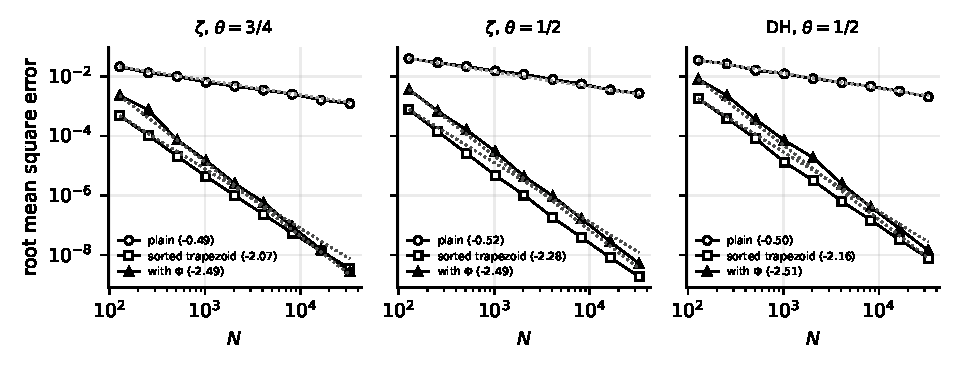
\includegraphics[width=\textwidth]{fig/bsy_halfdisk.pdf}
\caption{Root mean square error against $N$ for the half disc identity (data of Table~\ref{bsy:tab:halfdisk}). The dotted lines have slopes $-\frac12$, $-2$ and $-\frac52$.}\label{bsy:fig:halfdisk}
\end{figure}

So the rates $N^{-4}$ and $N^{-5}$ are reached on the line by an exact local form of the criterion. For the whole line no such rate is proved (Open problem~\ref{bsy:op:line}).

\subsection{Truncation on the whole line}\label{bsy:sec:trunc}

\begin{resultpar}\label{bsy:res:tail}
On the line itself the Cauchy tail beyond a height can be bounded directly. Assume RH. Then
\[
\int_T^t\log|\zeta(\tfrac12+iu)|\,du=O\Bigl(\frac{\log t}{(\log\log t)^2}\Bigr)\qquad(3\le T\le t),
\]
the estimate behind Theorem~1.1 of Bui, Lester and Milinovich \cite{BLM14}. Let $A(t)$ be the left side with $T$ replaced by $t_0+T$ and $w=P_{1/2}(t_0-\cdot)$. Integration by parts gives $\int_{t_0+T}^\infty\log|\zeta(\frac12+i\tau)|\,w(\tau)\,d\tau=-\int_{t_0+T}^\infty A(\tau)w'(\tau)\,d\tau$, since $A(t)w(t)\to0$, and $w'(\tau)=O_{t_0}(\tau^{-3})$. With the same bound below $t_0-T$,
\[
\int_{|\tau-t_0|>T}\log|\zeta(\tfrac12+i\tau)|\,P_{1/2}(t_0-\tau)\,d\tau=O_{t_0}\Bigl(\frac{\log T}{T^2(\log\log T)^2}\Bigr)
\]
(conditional on RH). At $t_0=0$ this is \cite[Theorem~1.1]{BLM14}, where it is also shown that the tail is not $O(T^{-2})$. At a level $\theta\in(\frac12,1)$, under RH, the integral of $\log\zeta$ around the rectangle with vertices $\theta+iT$, $\theta+it$ and $+\infty$ bounds the primitive of $\log|\zeta(\theta+iu)|$ by $O_\theta(\log t)$, and the tail by $O_\theta(T^{-2}\log T)$.
\end{resultpar}

For the rule place $N=2T/h$ nodes $\tau_j=t_0-T+h(j+U)$, $0\le j<N$, with one shift $U$ uniform on $[0,1)$. At $\theta=\frac34$ nothing is deflated. At $\theta=\frac12$ deflate each zero $\rho_k=\frac12+i\gamma_k$ with $|\gamma_k-t_0|\le T+1$ by
\[
u_k(s)=\log\Bigl|\frac{(s-\rho_k)(s-\rho_k+2)}{(s-\rho_k+1)^2}\Bigr|,
\]
which is harmonic on $\Re s>\frac12$ and $O(|s|^{-2})$; on the line it is $\frac12\log\frac{x^2(4+x^2)}{(1+x^2)^2}$ with $x=\tau-\gamma_k$, about $x^{-2}$ for large $|x|$, and its integral over $\R$ is $0$. The estimate is $h\sum_j\bigl[(f-\sum_ku_k)P\bigr](\tau_j)+\sum_k\int_{|\tau-t_0|\le T}u_kP\,d\tau$, the window means of the $u_k$ computed by quadrature. The shifted grid is unbiased for the integral over the window. Adding back instead the whole line means $u_k(1+it_0)$ would add the tails $\sum_k\int_{|\tau-t_0|>T}u_kP\,d\tau$, about the value of $P$ at the edge times the sum of the reciprocal distances of the zeros to the edges; for this variant at $\theta=\frac12$ the measured $T^2\cdot|\mathrm{error}|$ grows from $0.15$ at $T=10$ to $1.24$ at $T=640$, more than $97$ percent of the error at $T=640$ being the deflation tails (computed), so it is not the tail of $\log|\zeta|$.

\begin{table}[h]
\centering\footnotesize\setlength{\tabcolsep}{3pt}
\begin{tabular}{rccccccc}
\toprule
 & \multicolumn{3}{c}{$\theta=\frac34$, $h=0.02$} & \multicolumn{4}{c}{$\theta=\frac12$, $h=0.01$, zeros deflated}\\
$T$ & error & spread & $T^2\cdot|\mathrm{error}|$ & error & spread & $T^2\cdot|\mathrm{error}|$ & zeros\\
\midrule
10 & $-9.47\times10^{-4}$ & $5.5\times10^{-8}$ & $0.095$ & $-2.09\times10^{-3}$ & $8.1\times10^{-7}$ & $0.209$ & 10\\
40 & $-3.40\times10^{-5}$ & $2.2\times10^{-8}$ & $0.054$ & $-5.37\times10^{-5}$ & $1.3\times10^{-8}$ & $0.086$ & 33\\
160 & $+4.36\times10^{-6}$ & $9.8\times10^{-9}$ & $0.112$ & $+1.05\times10^{-5}$ & $9.4\times10^{-9}$ & $0.268$ & 123\\
640 & $+6.47\times10^{-8}$ & $8.2\times10^{-10}$ & $0.027$ & $+7.84\times10^{-8}$ & $5.5\times10^{-10}$ & $0.032$ & 742\\
1280 & $-1.36\times10^{-7}$ & $1.8\times10^{-10}$ & $0.223$ & & & & \\
\bottomrule
\end{tabular}
\caption{Truncated Cauchy average of $\log|\zeta(\theta+i\tau)|$ over $|\tau-t_0|\le T$ at $t_0=85.7$, minus $\log|h_\theta(1+it_0)|$; as in Remark~\ref{bsy:rem:local}, the zeros above $3\times10^{12}$ move the whole line average away from $\log|h_\theta(1+it_0)|$ by less than $10^{-12}$, with no hypothesis. Mean error and spread over $10$ random shifts of the grid (computed, floating point). At $\theta=\frac12$ the zeros with $|\gamma-t_0|\le T+1$ (the zero range convention, counted in the last column) are deflated and their window means added back (the unbiased rule). The shifted grid is unbiased for the window integral, so the mean error is minus the Cauchy tail beyond $T$, up to the spread. In this range $T^2\cdot|\mathrm{error}|$ stays below $0.27$; the bounds of \cite{BLM14} allow slow growth.}\label{bsy:tab:trunc}
\end{table}

In Table~\ref{bsy:tab:trunc} the measured error is the tail, which under RH is $O(T^{-2}\log T)$, that is $O(N^{-2}\log N)$ at a fixed step, and the spread over the shifts is at most $8.1\times10^{-7}$ (at $T=10$, $\theta=\frac12$) and below $1.0\times10^{-8}$ for $T\ge160$. The error changes sign with $T$ (between $T=40$ and $160$ and again, at $\theta=\frac34$, between $640$ and $1280$), a bounded oscillation of $T^2\cdot|\mathrm{error}|$ consistent with $T^{-2}$ up to logarithms in this range (computed). This is computed, not a theorem: at a fixed step the discretisation error of one shift need not tend to $0$ as $T$ grows (besides an endpoint term of order $h$ times the integrand at the edges of the window, it contains an aliasing term, of order $e^{-2\pi b/h}$ for an integrand analytic in a strip of width $b$, which in general does not decay as $T$ grows), so a rate in $N$ needs bounds on the deflated integrand, or a step that shrinks with $N$ (Open problem~\ref{bsy:op:line}). The tail is bounded under RH, not corrected.

With no hypothesis, Bui, Lester and Milinovich \cite[Theorem~1.2]{BLM14} prove that for $T\ge3$
\[
I(T)=\int_{-T}^T\frac{\log|\zeta(\frac12+it)|}{\frac14+t^2}\,dt=2\pi\sum_{\substack{|\gamma|\le T\\ \beta>1/2}}\log\Bigl|\frac{\rho}{1-\rho}\Bigr|+O\Bigl(\frac{\log T}{T^2}\Bigr):
\]
up to that error the truncated integral is the sum over the zeros below height $T$. With Theorem~\ref{bsy:thm:bsy} the tail is $I(\infty)-I(T)=2\pi\sum_{|\gamma|>T,\,\beta>1/2}\log|\rho/(1-\rho)|+O(\log T/T^2)$, which is $O(\log T/T)$ with no hypothesis, since each term lies between $0$ and $(2\beta-1)/(2|1-\rho|^2)\le1/(2\gamma^2)$ and there are $O(T\log T)$ zeros up to height $T$. Under RH their Omega theorem disproves the conjecture $I(T)=O(T^{-2})$ of Borwein, Bradley and Crandall \cite{BBC00}, as stated in \cite{BLM14}.

\subsection{Scanning heights}

The local criterion invites a scan over $t_0$. Chapter~\ref{chap:cf} provides the particle filter along the Cauchy flow (Section~\ref{cf:sec:pf}) and nested sampling over heights (Section~\ref{cf:sec:ns}), with the results of Tables~\ref{cf:tab:scan} and~\ref{cf:tab:ns}. Once a suspicious height is found, the defect $D_\theta(t_0)$ of Theorem~\ref{bsy:thm:bsy} gives a check, in floating point: centred at a zero at distance $\delta$ to the right of the line $\Re s=\theta$ it is at least $\log\frac{1-\theta+\delta}{1-\theta-\delta}\approx\frac{2\delta}{1-\theta}$.
